\subsection{Modelled systems}

\begin{frame}
 \frametitle{The modelled systems}
 \begin{itemize}
  \item Quantum dots
  \begin{itemize}
  \item Two dimensions
  \item Three dimensions
  \item Double wells
  \end{itemize}
  \pause
  \item Atomic systems
  \begin{itemize}
  \item Atoms
  \item Homonuclear Diatomic Molecules
  \end{itemize}
 \end{itemize}
\end{frame}

\begin{frame}
 \frametitle{Quantum dots}
 
 Quantum dots are interacting electrons in a harmonic oscillator potential
 
 \begin{equation}
  V_\mathrm{ext}(\mathbf{r}) = \frac{1}{2}\omega^2r^2,
 \end{equation}
 
 where $\omega$ is the oscillator frequency.
 
 \pause
 
 The harmonic oscillator eigenfunctions are
 
 \begin{equation}
  \phi_{n_x, n_y, n_z}(\mathbf{r}) = H_{n_x}(\sqrt{\omega}x)H_{n_y}(\sqrt{\omega}y)H_{n_z}(\sqrt{\omega}z)e^{-\frac{1}{2}\omega r^2},
 \end{equation}
 
 where $H_n(x)$ is the $n$'th level Hermite polynomial.


 
\end{frame}

\begin{frame}
 \frametitle{Quantum dots}
 
 Introducing a variational parameter $\alpha$ yields
 
 \begin{equation}
  \phi_{n_x, n_y, n_z}(\mathbf{r}; \alpha) = H_{n_x}(kx)H_{n_y}(ky)H_{n_z}(kz)e^{-\frac{1}{2}k^2r^2},
 \end{equation}
 
 where $k = \sqrt{\alpha\omega}$ represents the scaled oscillator potential.
 \shift

 \textbf{Problem}: With the electron-electron interaction these are no longer eigenfunctions of the Hamiltonian.
 \shift
 
 \textbf{Solution}: Quantum Monte-Carlo!
 
\end{frame}

\begin{frame}
 \begin{figure}
 \begin{center}
  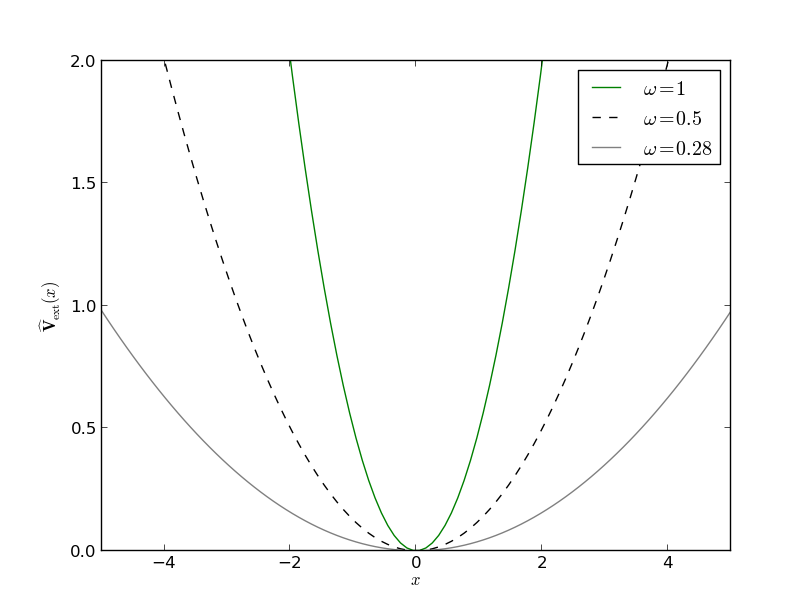
\includegraphics[scale=0.4]{../graphics/Potentials/qdots.png}
  \caption{A one-dimensional version of the single-particle potential of quantum dots.}
  \label{fig:extPotQDOTS}
 \end{center}
\end{figure}
\end{frame}

\begin{frame}
 \frametitle{Double wells}
 
 The double-well potential used is
 
 \begin{equation}
  V_\mathrm{ext}(\mathbf{r}) = \frac{1}{2}m^\ast \omega_0^2 \left[r^2 + \frac{1}{4}R^2 - R|x|\right], 
 \end{equation}

 where $R$ is the well separation, and $m^\ast$ and $\omega_0$ are material constants.
 \shift
 
 The construction of the new basis will be discussed later.
 
\end{frame}

\begin{frame}
 \begin{figure}
 \begin{center}
  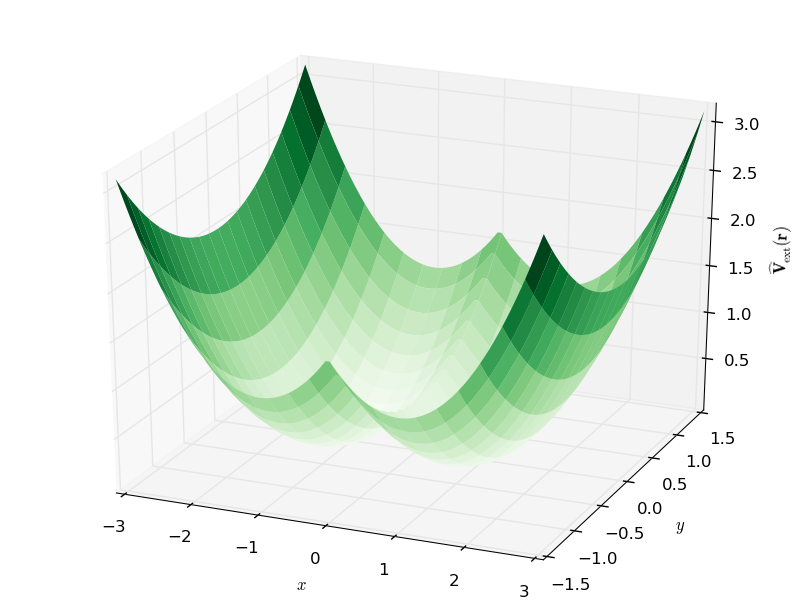
\includegraphics[scale=0.4]{../graphics/Potentials/doubleWell.png}
  \caption{The external potential for a double-well quantum dot.}
  \label{fig:extPotDoubleWell}
 \end{center}
\end{figure}
\end{frame}

\begin{frame}
 \frametitle{Atomic systems}
 
 Atomic systems are interacting electrons surrounding opposite charged nuclei. In the case of atoms, there is a single nucleus with charge $Z=N$. The potential used is
 
 \begin{equation}
 V_\mathrm{ext}(\mathbf{r}) = -\frac{Z}{r}. \label{eq:v0hydro}
\end{equation}
 \shift
 
 This corresponds to the hydrogen atom potential with the \textit{Born-Oppenheimer Approximation}.
 
\end{frame}

\begin{frame}
\begin{figure}
 \begin{center}
  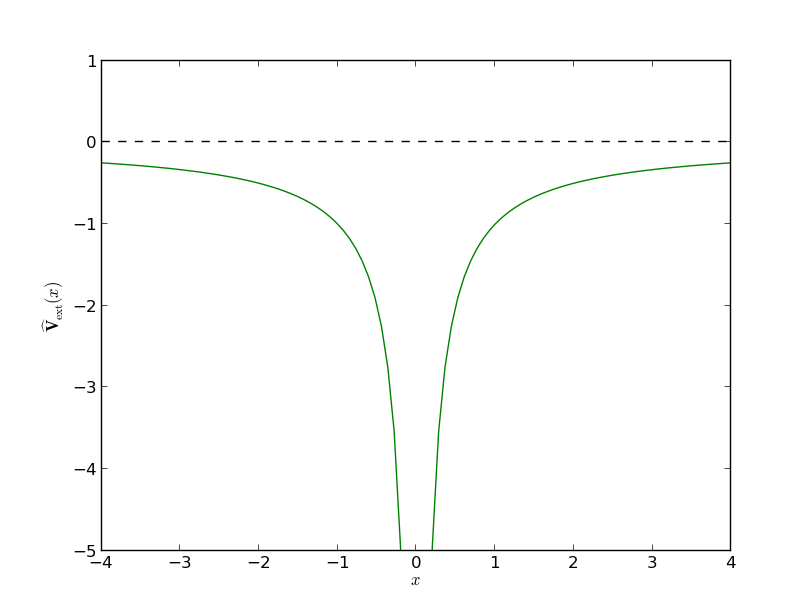
\includegraphics[scale=0.4]{../graphics/Potentials/hydrogen.png}
  \caption{The one-dimensional version of the single-particle potential of hydrogen.}
  \label{fig:extPotHydrogen}
 \end{center}
\end{figure}
\end{frame}

\begin{frame}
 The eigenfunctions are
 
 \begin{equation*}
 \phi_{nlm}(r, \theta, \phi; Z) \propto r^l e^{-Zr/n}\left[L_{n-l-1}^{2l+1}\left(\frac{2r}{n}Z\right)\right] Y_l^m(\theta, \phi), 
\end{equation*}

where $L_{q-p}^p(x)$ are the \textit{associated Laguerre polynomials} and $Y_l^m(\theta, \phi)$ are the \textit{spherical harmonics}. 
\shift
The spherical harmonics are related to the \textit{associated Legendre functions} $P_l^m$ in the following manner:

\begin{equation}
 Y_l^m(\theta, \phi) \propto   P_l^m(\cos\theta)e^{im\phi}. \label{eq:spherHarm}
\end{equation}

\end{frame}

\begin{frame}
 \textbf{Problem}: The spherical harmonics are complex functions. 
 \shift
 \textbf{Solution}: Use a special superposition of spherical harmonics known as the real-valued \textit{solid harmonics}
 
 \begin{align}
S_l^m(r, \theta, \phi) &\propto r^l\left[Y_l^m(\theta, \phi) + (-1)^m Y_l^{-m}(\theta, \phi)\right] \\
 &\propto r^{l} P_l^{|m|}(\cos\theta) \begin{cases} \cos m\phi & m \ge 0 \\ \sin|m|\phi &  m < 0 \end{cases}.     
\end{align}

 \end{frame}
 
 \begin{frame}
  The resulting eigenfunctions become 
  
\begin{equation*}
  \phi_{nlm}(r, \theta, \phi; k) \propto e^{-kr/n}\left[L_{n-l-1}^{2l+1}\left(\frac{2r}{n}k\right)\right] S_l^m(r, \theta, \phi) \equiv \phi^\mathrm{H}_{nlm}(\mathbf{r}), 
\end{equation*}

where $k = \alpha Z$ is a scaled charge with $\alpha$ as a variational parameter.
 \end{frame}

\begin{frame}
 \frametitle{Molecules}
 
 The Hamiltonian describing the homonuclear diatomic molecules is
 
 \begin{equation*}
 \OP{H}_{\mathrm{Mol.}}(\mathbf{r}, \mathbf{R}) = \sum_{i=1}^N \left[-\frac{1}{2}\nabla_i^2 + \frac{Z}{|\mathbf{r}_i + \mathbf{R}/2|} + \frac{Z}{|\mathbf{r}_i - \mathbf{R}/2|}\right] + \frac{Z^2}{R} + \sum_{i<j} \frac{1}{r_{ij}},
\end{equation*}

where $Z=N/2$ is the charge of the nuclei, $\mathbf{R}$ is the vector between the nuclei and $\mathbf{r}_i$ is the coordinates of electron $i$.
 
\end{frame}

\begin{frame}
 \begin{figure}
 \begin{center}
  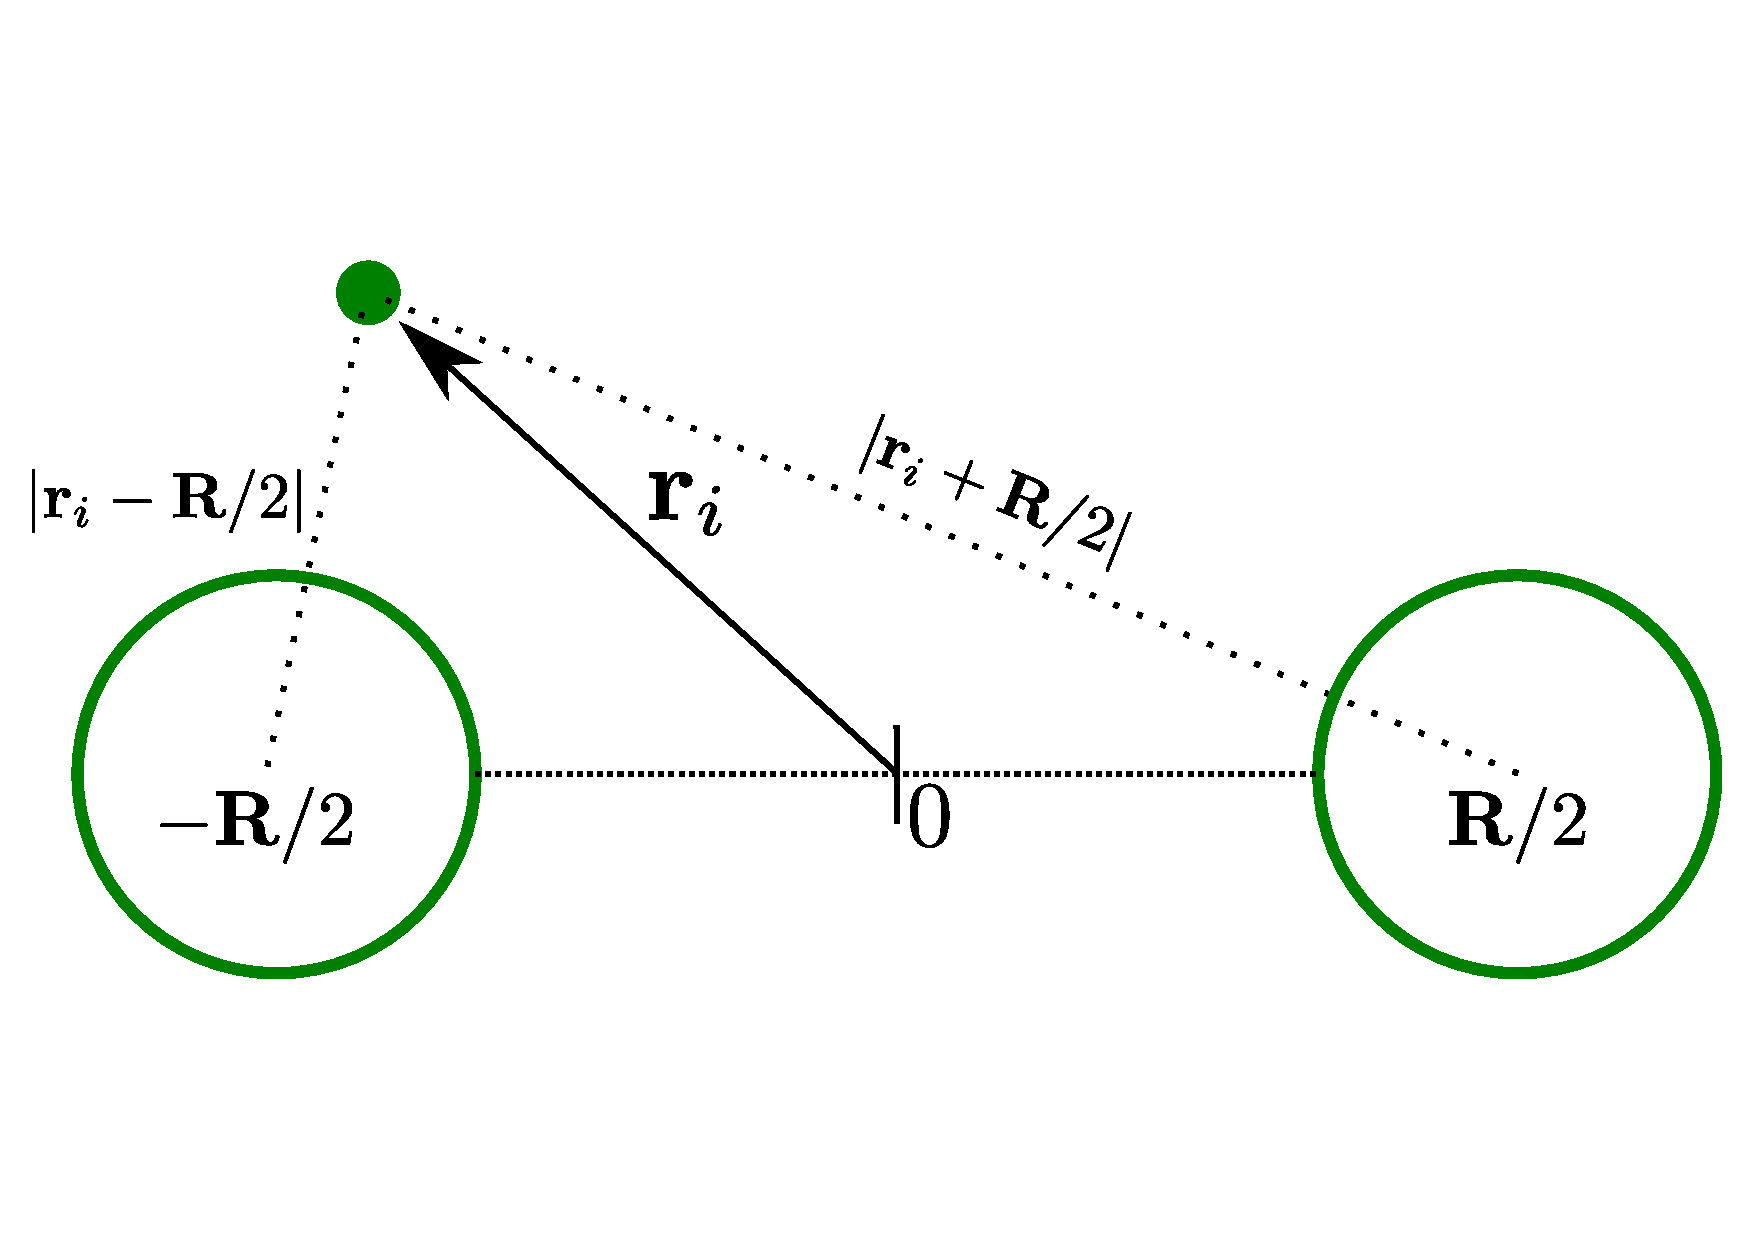
\includegraphics[scale=0.3]{../graphics/Molecules.pdf}
  \caption{The model for the diatomic molecule.}
 \end{center}
\end{figure}
\end{frame}

\begin{frame}
 In order to transform the hydrogen eigenstates $\phi_{nlm}^\mathrm{H}(\mathbf{r})$, which are symmetric around a single nucleus, into molecular single-particle states $\phi_{nlm}^\pm (\mathbf{r}_i)$, a superposition of the two mono-nucleus wave functions are used:

\begin{align*}
 \phi_{nlm}^+ (\mathbf{r}_i, \mathbf{R}) &= \phi_{nlm}^\mathrm{H}(\mathbf{r}_i + \mathbf{R}/2) + \phi_{nlm}^\mathrm{H}(\mathbf{r}_i - \mathbf{R}/2)\label{eq:moleculeTransPlus}, \\
 \phi_{nlm}^- (\mathbf{r}_i, \mathbf{R}) &= \phi_{nlm}^\mathrm{H}(\mathbf{r}_i + \mathbf{R}/2) - \phi_{nlm}^\mathrm{H}(\mathbf{r}_i - \mathbf{R}/2)\label{eq:moleculeTransMin}.
\end{align*}
\shift 

The same transformation are used to transform the harmonic oscillator eigenfunctions into the double well basis.

\end{frame}



